\documentclass[10pt,a4paper]{article}

% ---------- Page geometry ----------
\usepackage[a4paper,margin=1in]{geometry}

% ---------- Fonts & encoding ----------
\usepackage[T1]{fontenc}
\usepackage[utf8]{inputenc}
\usepackage{lmodern}
\usepackage{microtype}          % better typography (protrusion, expansion)

% ---------- Math ----------
\usepackage{amsmath,amssymb,amsfonts}
\usepackage{mathtools}

% ---------- Graphics & tables ----------
\usepackage{graphicx}
\usepackage{booktabs}           % professional tables
\usepackage{float}              % add to preamble
\usepackage{multirow}
\usepackage{caption}
\captionsetup{font=small,labelfont=bf}

% ---------- Two-column layout ----------
\usepackage{multicol}
\setlength{\columnsep}{0.25in}

% ---------- Colors & links ----------
\usepackage{xcolor}
\usepackage[colorlinks=true,
            linkcolor=blue!50!black,
            citecolor=green!40!black,
            urlcolor=blue!60!black]{hyperref}

% ---------- Misc ----------
\usepackage{enumitem}           % tight lists
\setlist{nosep}

% ---------- Title block spanning both columns ----------
\makeatletter
\newcommand{\twocoltitle}[1]{%
  \begin{@twocolumnfalse}
    \maketitle
    \vspace{-1em}
  \end{@twocolumnfalse}%
}
\makeatother

% ---------- Metadata ----------
\title{\textbf{On the stability of nonconvex Lp-IRLS as a robust regression method}}
\author{
  Ortiz Badenes, P. \thanks{ UPV, pablo.ortizbadenes@gmail.com}
}
\date{\today}

\begin{document}

% Full-width title block
\twocoltitle{}

% ---------- Abstract (full width) ----------
\begin{@twocolumnfalse}
\begin{abstract}
\noindent
$L_p$ regression, with $0<p<1$ has been studied as a robust linear regression method, as it downweights outliers, reducing the impact they have on the regression. A common implementation of this method is Iterative Reweighted Least Squares, which depends on 3 parameters. This article studies how near-optimal values for those parameters can be found if the underlying model is known, the stability of those parameters across perturbations in the contamination scenario, and a method to estimate the parameters off experimental data, to provide a practical tuning heuristic when the true model is unknown.
\end{abstract}
\vspace{0.5em}
\end{@twocolumnfalse}

% ---------- Two-column body ----------
\begin{multicols}{2}

\section{Introduction}
\label{sec:intro}

Ordinary least squares (OLS) is a natural estimator for linear regression
under Gaussian noise, but its squared-error objective gives large residuals
substantial influence. Robust regression methods address this sensitivity by
reducing the contribution of observations with large residuals. Classical
examples include Huber's robust estimator and iteratively reweighted
least-squares procedures \cite{huber1964, hollandwelsch1977}. A direct way to
reduce the leverage of large residuals is to replace the squared loss with an
$L_p$ loss with $0<p<1$: while the squared loss grows quadratically with
residual magnitude, $|r|^p$ grows sublinearly, so a large residual contributes 
less relative to a small one than it does under OLS. Strictly, this range
defines a nonconvex quasi-norm objective rather than a norm; its reduced
sensitivity comes with a more difficult optimization problem.

In order to avoid the problems of division by 0, the smoothed objective is studied
\[
  J(\boldsymbol{\beta};p,\delta)
  = \sum_{i=1}^{n}
    \left(r_i(\boldsymbol{\beta})^2+\delta^2\right)^{p/2},
  \qquad 0<p<1,
\]
where $r_i(\boldsymbol{\beta})$ is the residual, $p$ controls the loss shape,
and $\delta>0$ smooths the loss near zero. The derivative of each summand
with respect to its residual is proportional to
$r_i(r_i^2+\delta^2)^{(p-2)/2}$. Thus the objective can be viewed through a
residual-dependent weight $(r_i^2+\delta^2)^{(p-2)/2}$: for large residuals,
this weight decreases approximately as $|r_i|^{p-2}$. The resulting
residual contribution grows approximately as $|r_i|^{p-1}$, rather than
linearly as in least squares. Outliers are therefore not discarded, but
their incremental influence on the fit is reduced.

IRLS is a natural computational implementation because, at each iteration,
these residual-dependent weights turn the update into a weighted least
squares problem. Solving that familiar subproblem updates the residuals and
therefore the weights, and the process repeats until a stopping criterion is
met. This connects the robust loss directly to an efficient linear
least-squares solver \cite{hollandwelsch1977}; the derivation and the
smoothed weights used here are given in Section~\ref{sec:method}. For
$p<1$, however, the objective is nonconvex, so IRLS is an iterative
optimization procedure rather than a guarantee of finding a global
minimizer. Its result and computational cost depend on the exponent $p$,
smoothing parameter $\delta$, initialization, and stopping tolerance
$\tau$. Related IRLS methods have also been studied for nonconvex objectives
in sparse recovery \cite{daubechies2010}. How to select these settings
together for regression under a specified contamination regime—and whether
they remain useful when the model or regime changes—are the questions
considered here.

The study focuses on severe response contamination: a proportion $\rho$ of
observations receives an additional perturbation whose scale $A$ is large
relative to the standard deviation $\sigma$ of the clean Gaussian noise.
Thus, the article doesn't claim that IRLS should dominate OLS in every setting;
OLS is expected to remain a strong baseline when contamination is small.
Instead, the primary question is whether a tuning procedure can identify useful
$(p,\delta,\tau)$ values for a known model and contamination regime, and
whether the resulting parameter choices can be reused. OLS and Huber
regression provide nonrobust and robust reference estimators, respectively;
the central contribution is the investigation of tuning and transfer rather
than a general claim of superiority over established robust estimators.

A key design choice is how performance is measured. Each estimator is fitted
to the contaminated training sample, but its coefficients are evaluated
against the known data-generating coefficients. This parameter-recovery
criterion tests recovery of the underlying signal: at exact coefficient
recovery, the error is zero, irrespective of the particular noise realization.
By contrast, evaluating only on observations after removing outliers would
primarily measure prediction on clean observations and would not directly
establish recovery of the generating model. Since both the Gaussian noise and
the contamination are random, comparisons use repeated experiments and
report average performance and its variability, as a single repetition will not
return significant results.

\section{Hypotheses}
\label{sec:hypotheses}

The investigation tests five empirical hypotheses:
\begin{enumerate}[label=\textbf{H\arabic*:}, leftmargin=*]
  \item Given a known model, contamination regime, and exact recovery metric,
  a computational search can jointly tune $p$, $\delta$, and $\tau$, yielding
  an oracle map from regimes and models to parameter settings.
  \item In severe-contamination settings, IRLS with tuned parameters
  outperforms OLS. This is an auxiliary comparison, not the paper's principal
  contribution.
  \item For a fixed contamination regime, tuned parameters are locally
  optimal across nearby models and thus depend primarily on the contamination
  regime rather than on the precise model.
  \item Parameters selected at an anchor regime remain effective at nearby
  contamination levels and magnitudes.
  \item An estimated contamination regime can be used to select approximate
  parameter settings from the oracle map without knowing the true model.
\end{enumerate}
The experiments assess recovery error across repeated samples and distinguish
tuning at a known regime from transfer to conditions not used for tuning.

The paper therefore studies the joint tuning of the IRLS settings, the local
stability and practical transferability of those settings, and finally model
parameter recovery. Its scope is deliberately narrower than a general
comparison of robust regression methods: it asks when computationally
tuned nonconvex $L_p$-IRLS can recover a known linear signal under severe
contamination, and what information is needed to choose and reuse its
parameters.

\section{Method}
\label{sec:method}
We consider a linear model with an intercept,
\[
  y_i = \mathbf{x}_i^\mathsf{T}\boldsymbol{\beta}+\eta_i,
  \qquad i=1,\ldots,n,
\]
where $\mathbf{x}_i$ includes a constant component and $\eta_i$ includes
both clean noise and vertical outlier contamination. Thus, $\eta_i$ is
completely determined by $(\sigma,\rho,A)$ which will be the contamination
regime, and $A\gg\sigma$. Given a training sample, the estimator minimizes the
smoothed $L_p$ residual objective
\begin{equation}
  \begin{aligned}
  J(\boldsymbol{\beta};p,\delta)
  = \sum_{i=1}^{n}
    \left(r_i(\boldsymbol{\beta})^2+\delta^2\right)^{p/2}
  \\
    r_i(\boldsymbol{\beta})
  = y_i-\mathbf{x}_i^\mathsf{T}\boldsymbol{\beta},
  \quad 0<p<1,\ \delta>0
  \label{eq:smoothed-lp}
  \end{aligned}
\end{equation}
The smoothing parameter prevents the residual-dependent weights from
diverging at zero. Differentiating the objective shows that a stationary
point satisfies weighted least-squares normal equations with weights
\begin{equation}
  w_i^{(t)}
  = \left((r_i^{(t)})^2+\delta^2\right)^{(p-2)/2},
  \quad
  r_i^{(t)}
  = y_i-\mathbf{x}_i^\mathsf{T}\boldsymbol{\beta}^{(t)}
  \label{eq:irls-weights}
\end{equation}
Accordingly, each IRLS iteration updates the coefficients by solving
\begin{equation}
  \boldsymbol{\beta}^{(t+1)}
  = \underset{\boldsymbol{\beta}}{\arg\min}
    \sum_{i=1}^{n} w_i^{(t)}
      \left(y_i-\mathbf{x}_i^\mathsf{T}\boldsymbol{\beta}\right)^2
  \label{eq:irls-update}
\end{equation}
Small residuals receive relatively large weights and large residuals receive
smaller weights, implementing the robust loss through a sequence of
least-squares solves. In the implementation, the initial coefficients are
the OLS estimate, and iterations stop when the relative change in the smoothed
objective falls below the tolerance $\tau$, or the iteration limit is reached.
Because $p<1$ makes the objective nonconvex, this procedure can depend on
initialization and does not in general certify a global minimum.

\section{Hypothesis 1}
\label{sec:H1}

The first hypothesis is that, when the generating model and contamination
regime are known, a computational search can jointly select $p$, $\delta$,
and $\tau$ for coefficient recovery. We use noise-aware Bayesian
optimization, which models the expensive, noisy tuning objective with a
Gaussian process and proposes candidates by expected improvement
\cite{jones1998,snoek2012}. Specifically, each candidate is evaluated on
repeated data sets; the sample variance of its mean recovery error is supplied
to a Mat\'ern-$5/2$ Gaussian-process model as observation noise. The next
candidate maximizes expected improvement over a pool of 512 points. The
exponent $p$ is searched linearly over $[0.4,0.9]$, while $\delta$ and the
stopping tolerance $\tau$ are searched logarithmically over $[10^{-6},10^{-1}]$
and $[10^{-10},10^{-1}]$, respectively. This follows the general Bayesian
optimization framework for expensive black-box objectives while accounting
for the variability of repeated measurements.

We test one known linear model with 1,000 observations, true coefficients
$\boldsymbol{\beta}=(1,1)$, a feature sampled uniformly from $[-2,2]$, and
Gaussian noise with standard deviation $\sigma=0.01$. Independently, each
response has probability $\rho=0.25$ of receiving Gaussian contamination
with standard deviation $A=10$. The search evaluates 15 initial candidates
and then 50 Bayesian-optimization proposals. Each candidate is scored by the
mean Euclidean coefficient-recovery error
$\|\hat{\boldsymbol{\beta}}-\boldsymbol{\beta}\|_2$ over 20 fixed-seed data
sets; the standard deviation across those replicates is also recorded.
Every fit is initialized by OLS and uses at most 200 IRLS iterations. The
lowest-error initial candidate and the final BO-selected candidate are
summarized in Table~\ref{tab:h1-results}.

\begin{table}[H]
  \centering
  \caption{Hypothesis 1 tuning results. Errors are mean $\pm$ standard
  deviation over 20 replicates.}
  \label{tab:h1-results}
  \scriptsize
  \resizebox{\columnwidth}{!}{%
  \begin{tabular}{lcccc}
    \toprule
    Candidate & $p$ & $\delta$ & $\tau$ & Recovery error \\
    \midrule
    Best initial & 0.4860 & $2.249\times10^{-2}$ & $3.477\times10^{-10}$
      & $(4.915\pm2.540)\times10^{-4}$ \\
    BO selected & 0.4029 & $1.672\times10^{-2}$ & $2.016\times10^{-10}$
      & $(4.902\pm2.693)\times10^{-4}$ \\
    \bottomrule
  \end{tabular}
  }
\end{table}

The BO-selected candidate was the lowest observed error among all 65
evaluations, but its mean error was only about 0.25\% below the best initial
candidate and the replicate variability was much larger than this difference.
Thus, this run demonstrates a practical joint search and a low-error setting
for the specified model and regime, but does not establish a meaningful
performance improvement over the initial design.

\begin{figure}[H]
  \centering
  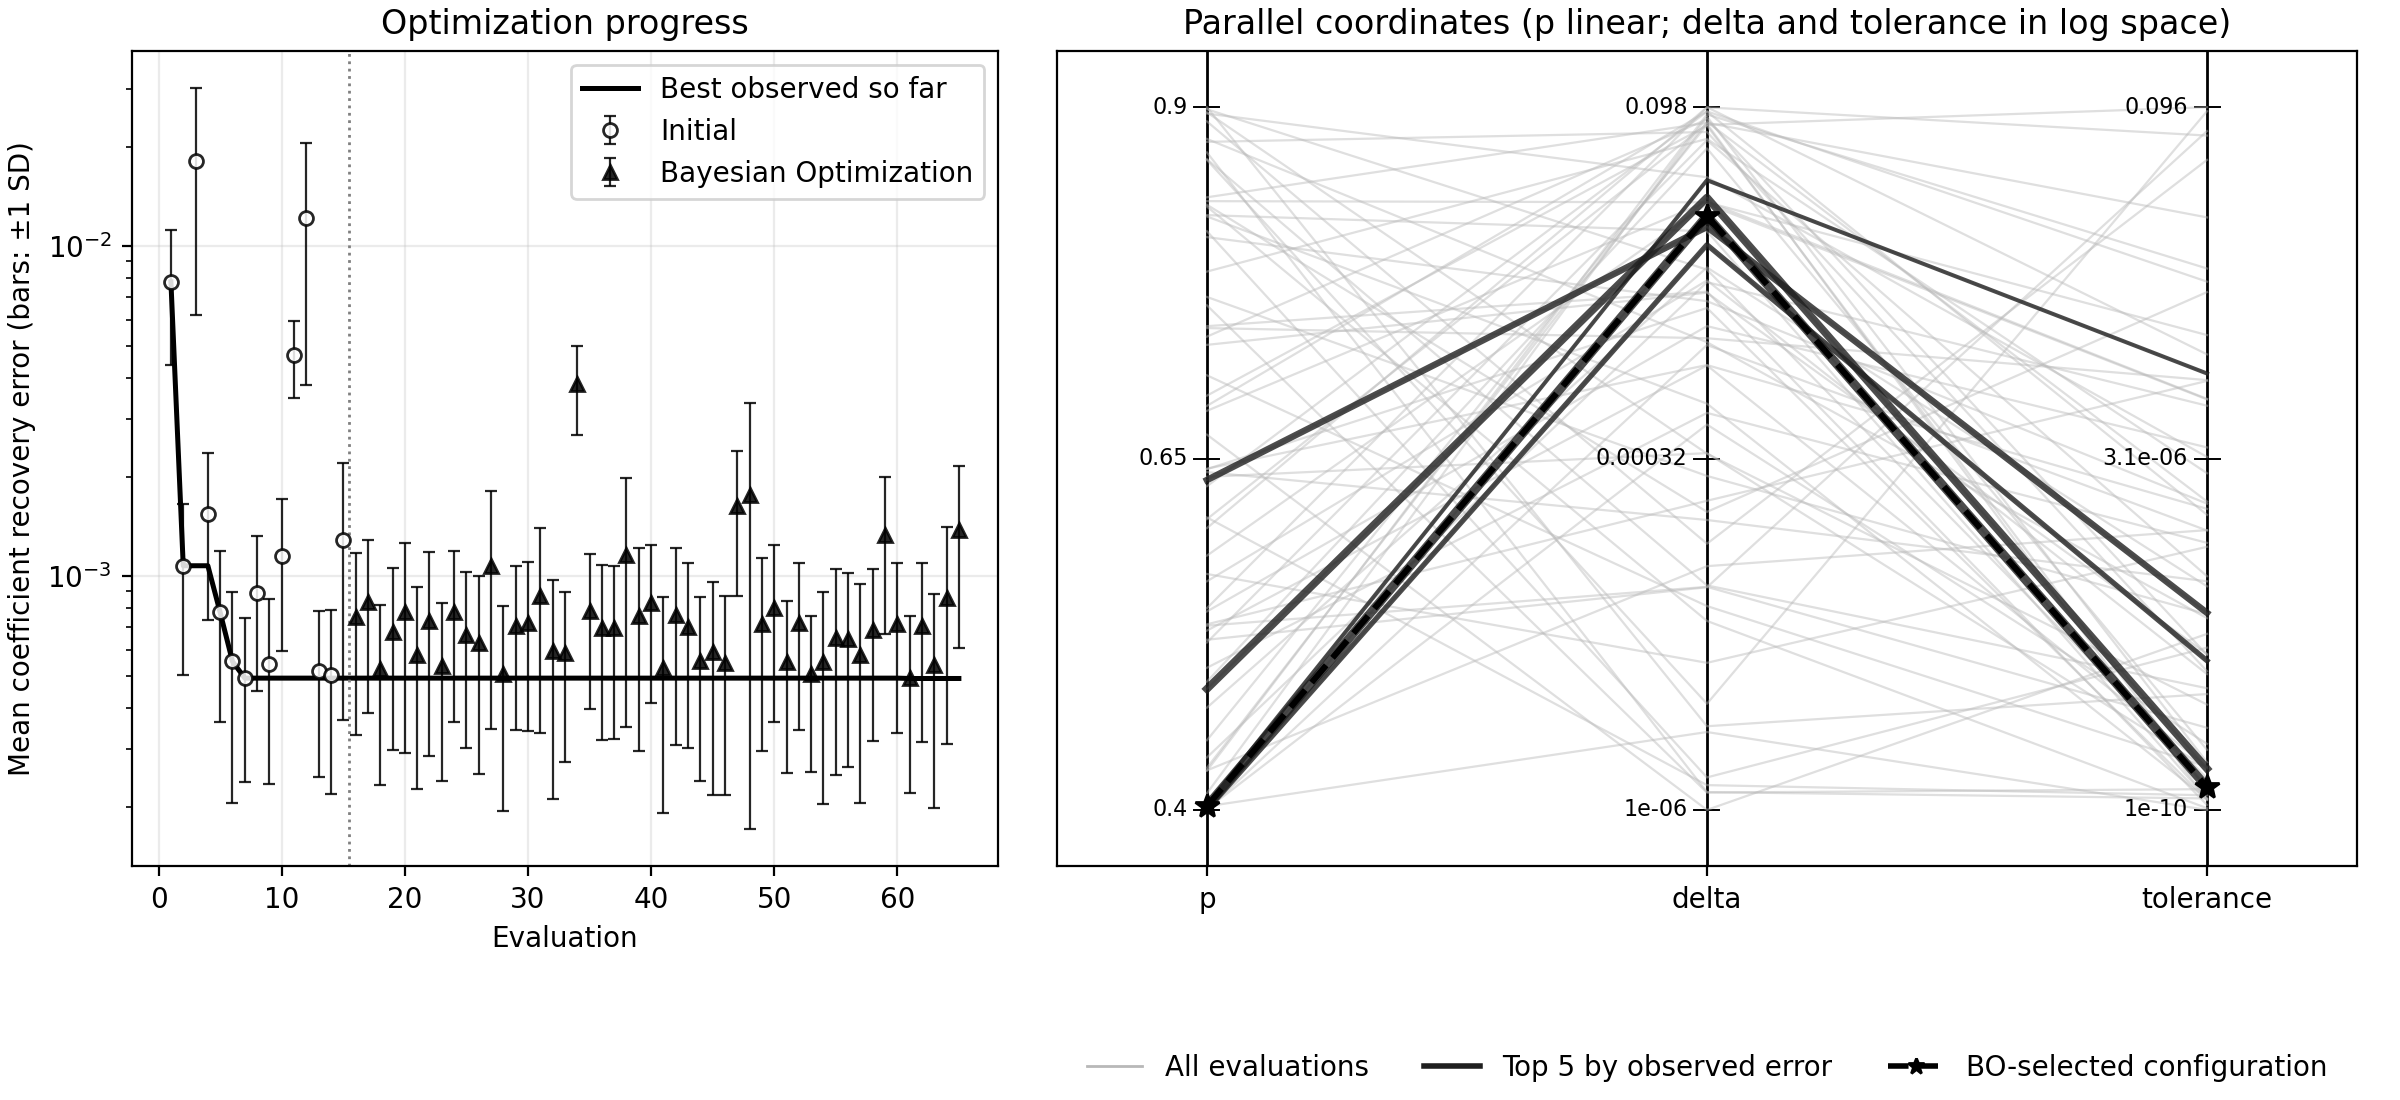
\includegraphics[width=\columnwidth]{../Assets/h1_comparison.png}
  \caption{Hypothesis 1 Bayesian-optimization evaluations. Left: mean
  coefficient-recovery error and $\pm1$ standard deviation by evaluation,
  with the best observed value to date. Right: evaluated parameter settings;
  the star marks the BO-selected candidate.}
  \label{fig:h1-bo-tuning}
\end{figure}

\section{Hypothesis 2}
\label{sec:H2}

Hypothesis 2 asks whether the H1-tuned $L_p$-IRLS estimator improves
coefficient recovery over OLS under severe response contamination. The methods
compared are OLS, Huber regression, and $L_p$-IRLS, all the same
data-generating model and contamination regime as in Hypothesis~1. For each of
1,000 independently generated data sets, all three methods are fitted to the
same sample. The feature, true coefficients, clean-noise standard deviation,
and contamination probability and scale are respectively sampled or set as
described in Section~\ref{sec:H1}. The $L_p$ estimator uses the H1-selected
values $p=0.4029$, $\delta=0.01672$, and $\tau=2.016\times10^{-10}$; each IRLS
fit is limited to 200 updates. Performance is the Euclidean
coefficient-recovery error $\|\hat{\boldsymbol{\beta}}-\boldsymbol{\beta}\|_2$.

For Huber regression, the transition threshold is fixed at
\[
  \delta_{\mathrm{H}} = 1.345\,\sigma
  = 1.345(0.01) = 0.01345.
\]
Here $\sigma$ is the known standard deviation of the uncontaminated Gaussian
noise, so $\delta_{\mathrm{H}}$ is expressed in the same response-residual
units. The factor $1.345$ is the conventional Huber choice giving about 95\%
asymptotic efficiency for Gaussian errors \cite{huber1964}. Residuals within
this threshold receive the quadratic loss, while larger residuals receive a
linear loss and are downweighted. This fixed, noise-based threshold is not
tuned to the outlier scale; it is also distinct from the $L_p$ smoothing
parameter $\delta$.

Across the 1,000 paired samples, mean recovery error (and standard deviation)
was $0.1837\ \pm 0.0980$ for OLS, $5.985\times10^{-4}\ \pm 3.186\times10^{-4}$
for Huber, and $4.420\times10^{-4}\ \pm 2.326\times10^{-4}$ for tuned
$L_p$-IRLS. Both robust estimators substantially reduced recovery error when
compared to OLS, supporting the hypothesis in this contamination regime. The
observed mean for tuned $L_p$-IRLS was lower than Huber's, but this experiment
is an auxiliary comparison and does not establish that $L_p$-IRLS is generally 
superior to Huber regression.

\begin{figure}[H]
  \centering
  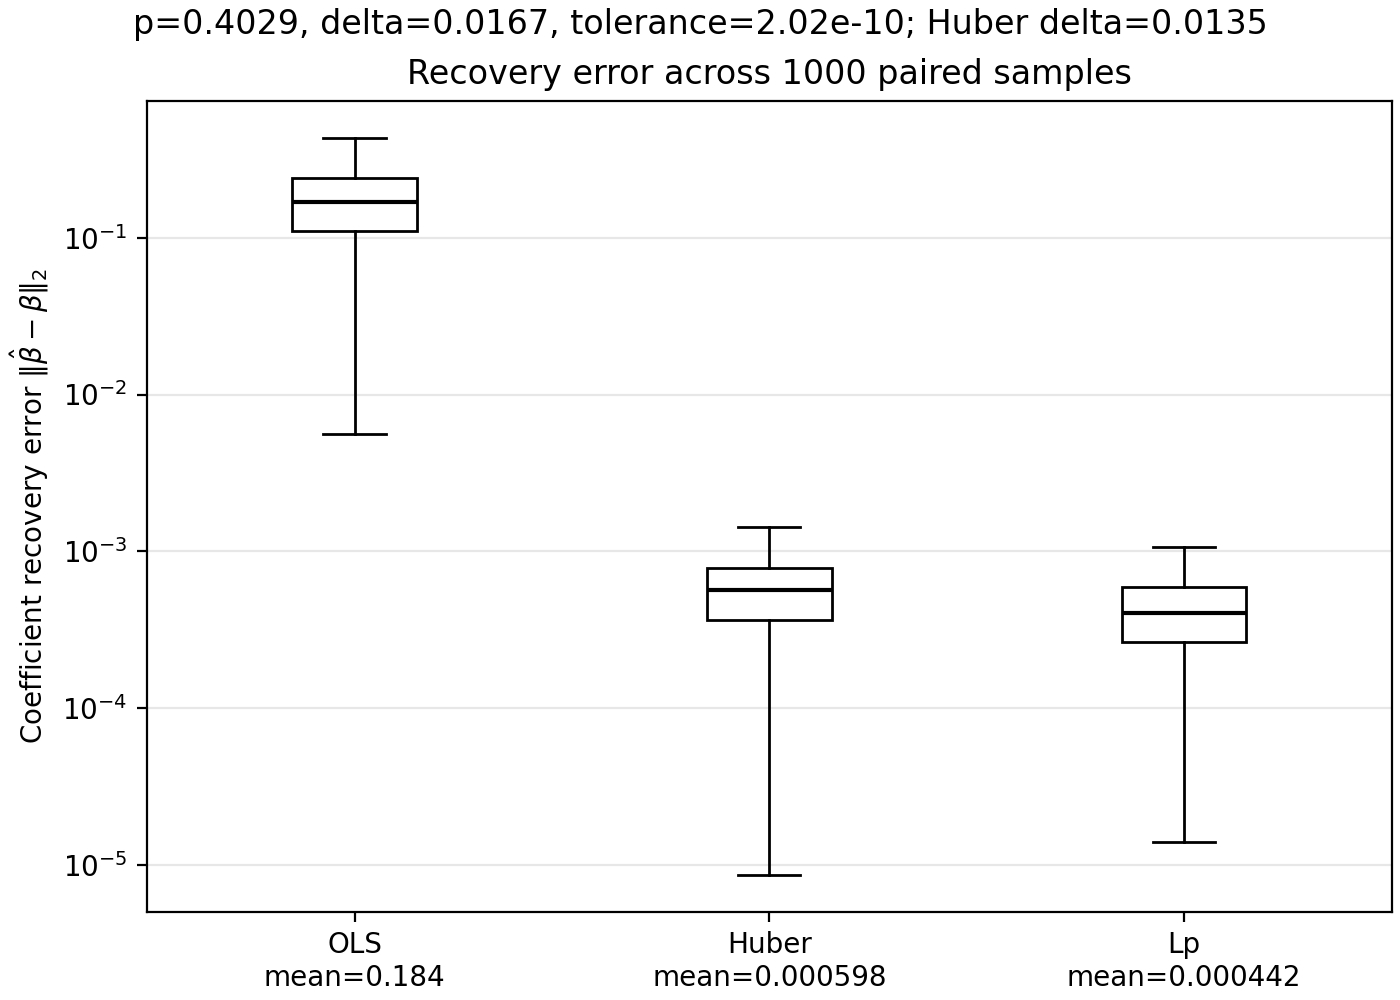
\includegraphics[width=\columnwidth]{../Assets/h2_comparison.png}
  \caption{Coefficient-recovery errors for OLS, Huber, and H1-tuned
  $L_p$-IRLS over 1,000 paired H2 samples. Boxes show the interquartile range
  and median; whiskers use the boxplot convention, and fliers are omitted.
  The vertical axis uses a symmetric log scale to show both the OLS errors
  and the much smaller errors of the robust estimators.}
  \label{fig:h2-comparison}
\end{figure}

\section{Hypothesis 3}
\label{sec:H3}

Hypothesis 3 evaluates whether the H1-tuned $L_p$-IRLS settings transfer to
nearby linear models when the contamination regime is held fixed. The anchor
model from Hypothesis~1, $\beta=(1,1)$, was rescaled on a $15\times15$ grid of
intercept and slope multipliers spanning $\pm20\%$ around the anchor value.
For each grid point, the H1-selected settings
$(p,\delta,\tau)=(0.4029, 1.672\times10^{-2}, 2.016\times10^{-10})$ were
applied without refitting, using $n=1000$, $\sigma=0.01$, $\rho=0.25$, and
$A=10$.

Each grid point was evaluated on 200 independently generated data sets,
using a distinct seed for every data set.

Performance was measured by the Euclidean coefficient-recovery error
$\|\hat{\boldsymbol{\beta}}-\boldsymbol{\beta}\|_2$. At the anchor model, the
mean error was $4.552\times10^{-4}$ with standard deviation
$2.423\times10^{-4}$. Across the grid, model-level mean errors ranged from
$4.055\times10^{-4}$ to $4.838\times10^{-4}$, and their standard deviations
ranged from $2.087\times10^{-4}$ to $2.655\times10^{-4}$. Relative to the
anchor, the largest absolute changes were 10.9\% in mean error and 13.9\% in
standard deviation. Recovery error remains of a similar order across the
tested neighborhood, with visible variation between grid points.

Because each grid point now uses independent data sets, these differences
reflect both changes in the generating coefficients and Monte Carlo
variability; the comparisons are not paired. The results are consistent with
the H1-tuned settings transferring reasonably across this neighborhood, but
do not establish that the settings are locally optimal: no alternative
settings were retuned and compared at each model.

\begin{figure}[H]
  \centering
  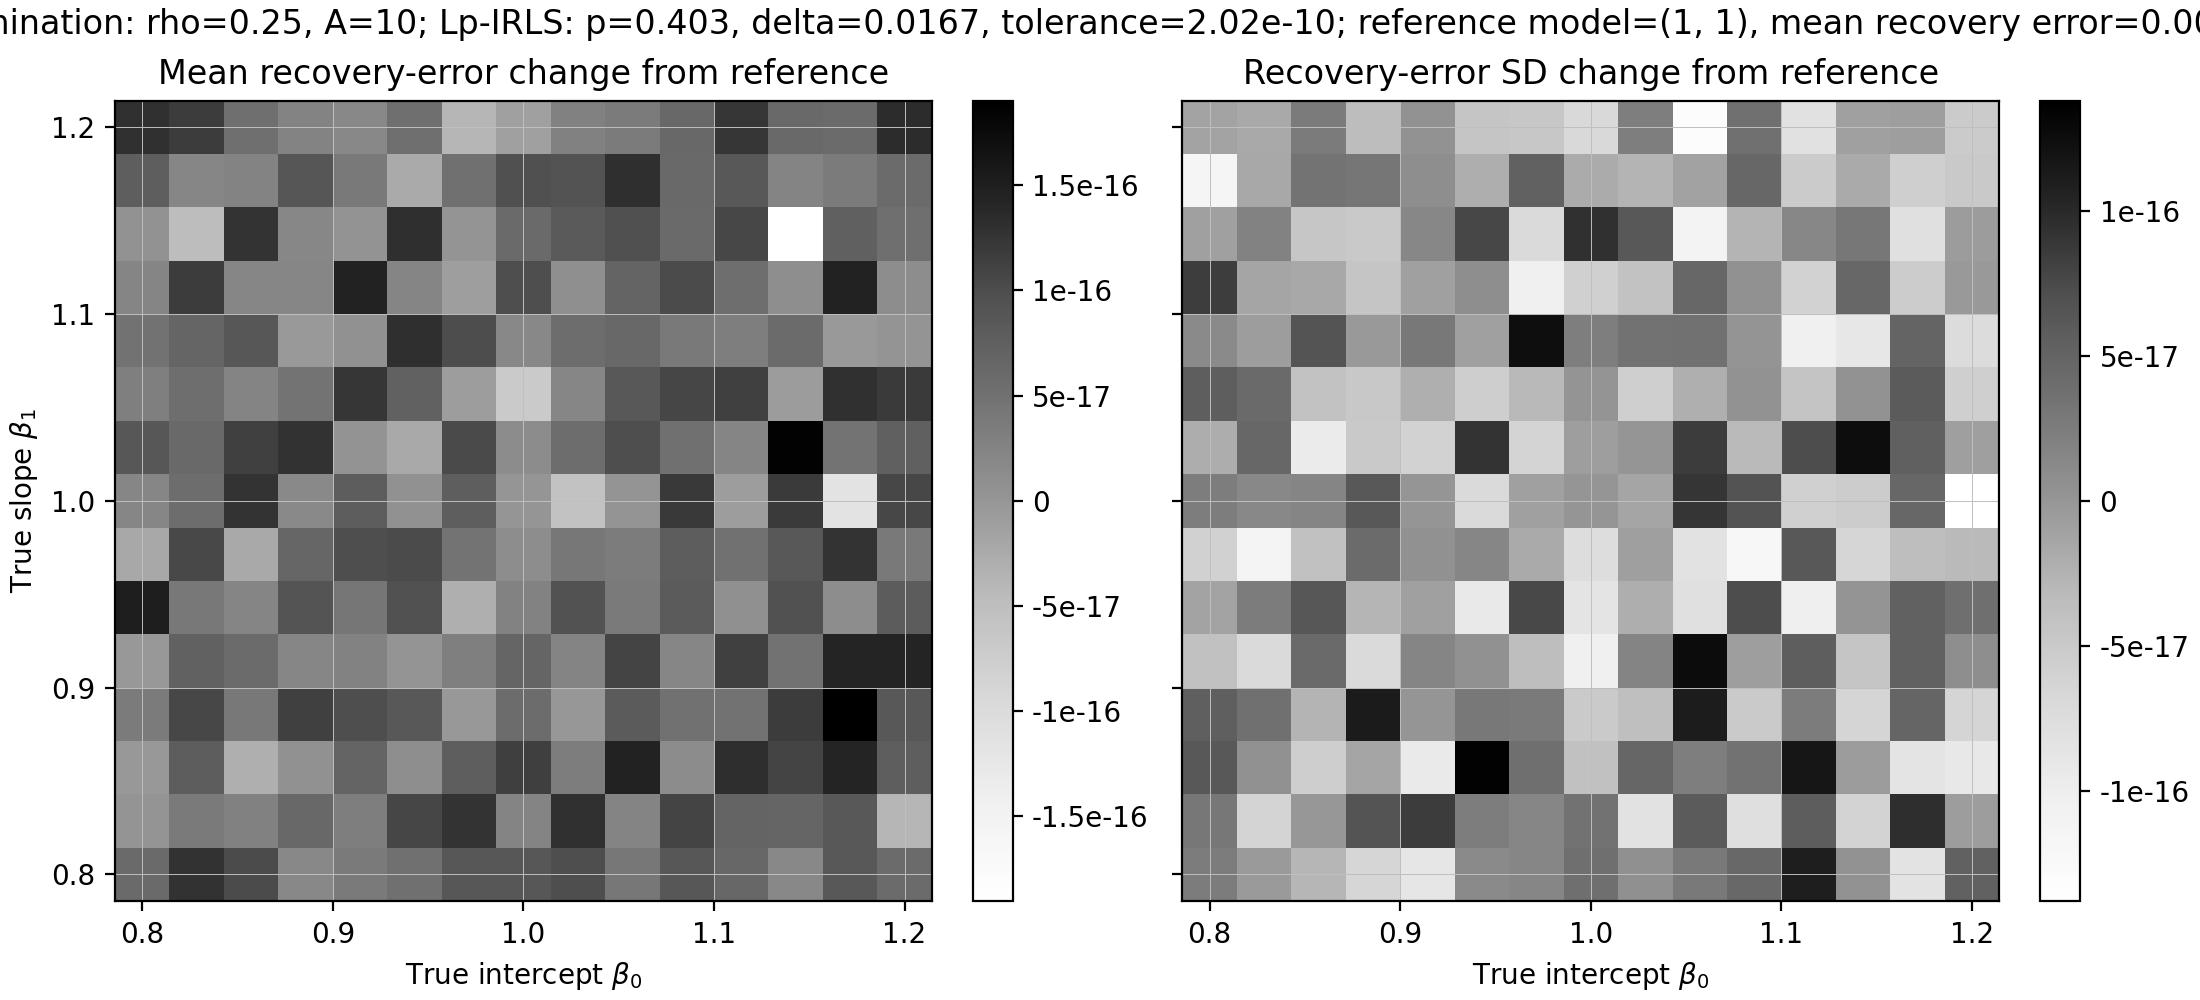
\includegraphics[width=\columnwidth]{../Assets/h3_comparison.png}
  \caption{Model-transfer experiment for the H1-tuned $L_p$-IRLS settings.
  Changes in mean coefficient-recovery error and its standard deviation
  relative to the anchor model are shown across a $15\times15$ grid near
  $\beta=(1,1)$. Each grid point uses 200 independently seeded data sets, so
  the differences include Monte Carlo variation as well as changes in the
  generating model.}
  \label{fig:h3-model-transfer}
\end{figure}

\section{Hypothesis 4}
\label{sec:H4}

Hypothesis 4 asks whether the H1-tuned $L_p$-IRLS settings remain effective
when the contamination regime varies around the anchor scenario rather than the
linear model. This is a practical transfer experiment: if the true outlier
proportion or amplitude differs within the tested range from the regime used
for training, can the selected hyperparameters still recover the underlying
coefficients without re-tuning? To test this, the anchor setting from
Hypothesis~1 was held fixed as the reference regime, and the contamination
pair $(\rho,A)$ was varied on a $15\times15$ grid. Specifically, the outlier
proportion was scaled by multipliers from $0.8$ to $1.2$ around the anchor
value $\rho_0=0.25$, spanning $\rho=0.20$ to $0.30$, while the outlier
amplitude was scaled by multipliers from $0.5$ to $10$ around $A_0=10$,
spanning $A=5$ to $100$. The H1-selected values,
$(p,\delta,\tau)=(0.4029,1.672\times 10^{-2},2.016\times 10^{-10})$, were
reused at every grid point, and each condition was replicated 200 times with
distinct sequential seeds across the grid.

The outcome was measured with the same coefficient-recovery error
$\|\hat{\boldsymbol{\beta}}-\boldsymbol{\beta}\|_2$ used throughout the
paper. The heatmaps in Figure~\ref{fig:h4-contamination-transfer} show the
change in mean recovery error and its standard deviation relative to values
bilinearly interpolated at the anchor contamination. Across the tested grid,
mean recovery error ranges from about $3.90\times 10^{-4}$ to
$4.93\times 10^{-4}$, compared with an interpolated anchor mean of
$4.44\times 10^{-4}$. The replicate standard deviation ranges from about
$1.96\times 10^{-4}$ to $2.66\times 10^{-4}$, compared with an interpolated
anchor standard deviation of $2.27\times 10^{-4}$. These results indicate
similar recovery across the tested contamination range, while not establishing
transfer to different outlier structures or contamination regimes outside it.

\begin{figure}[H]
  \centering
  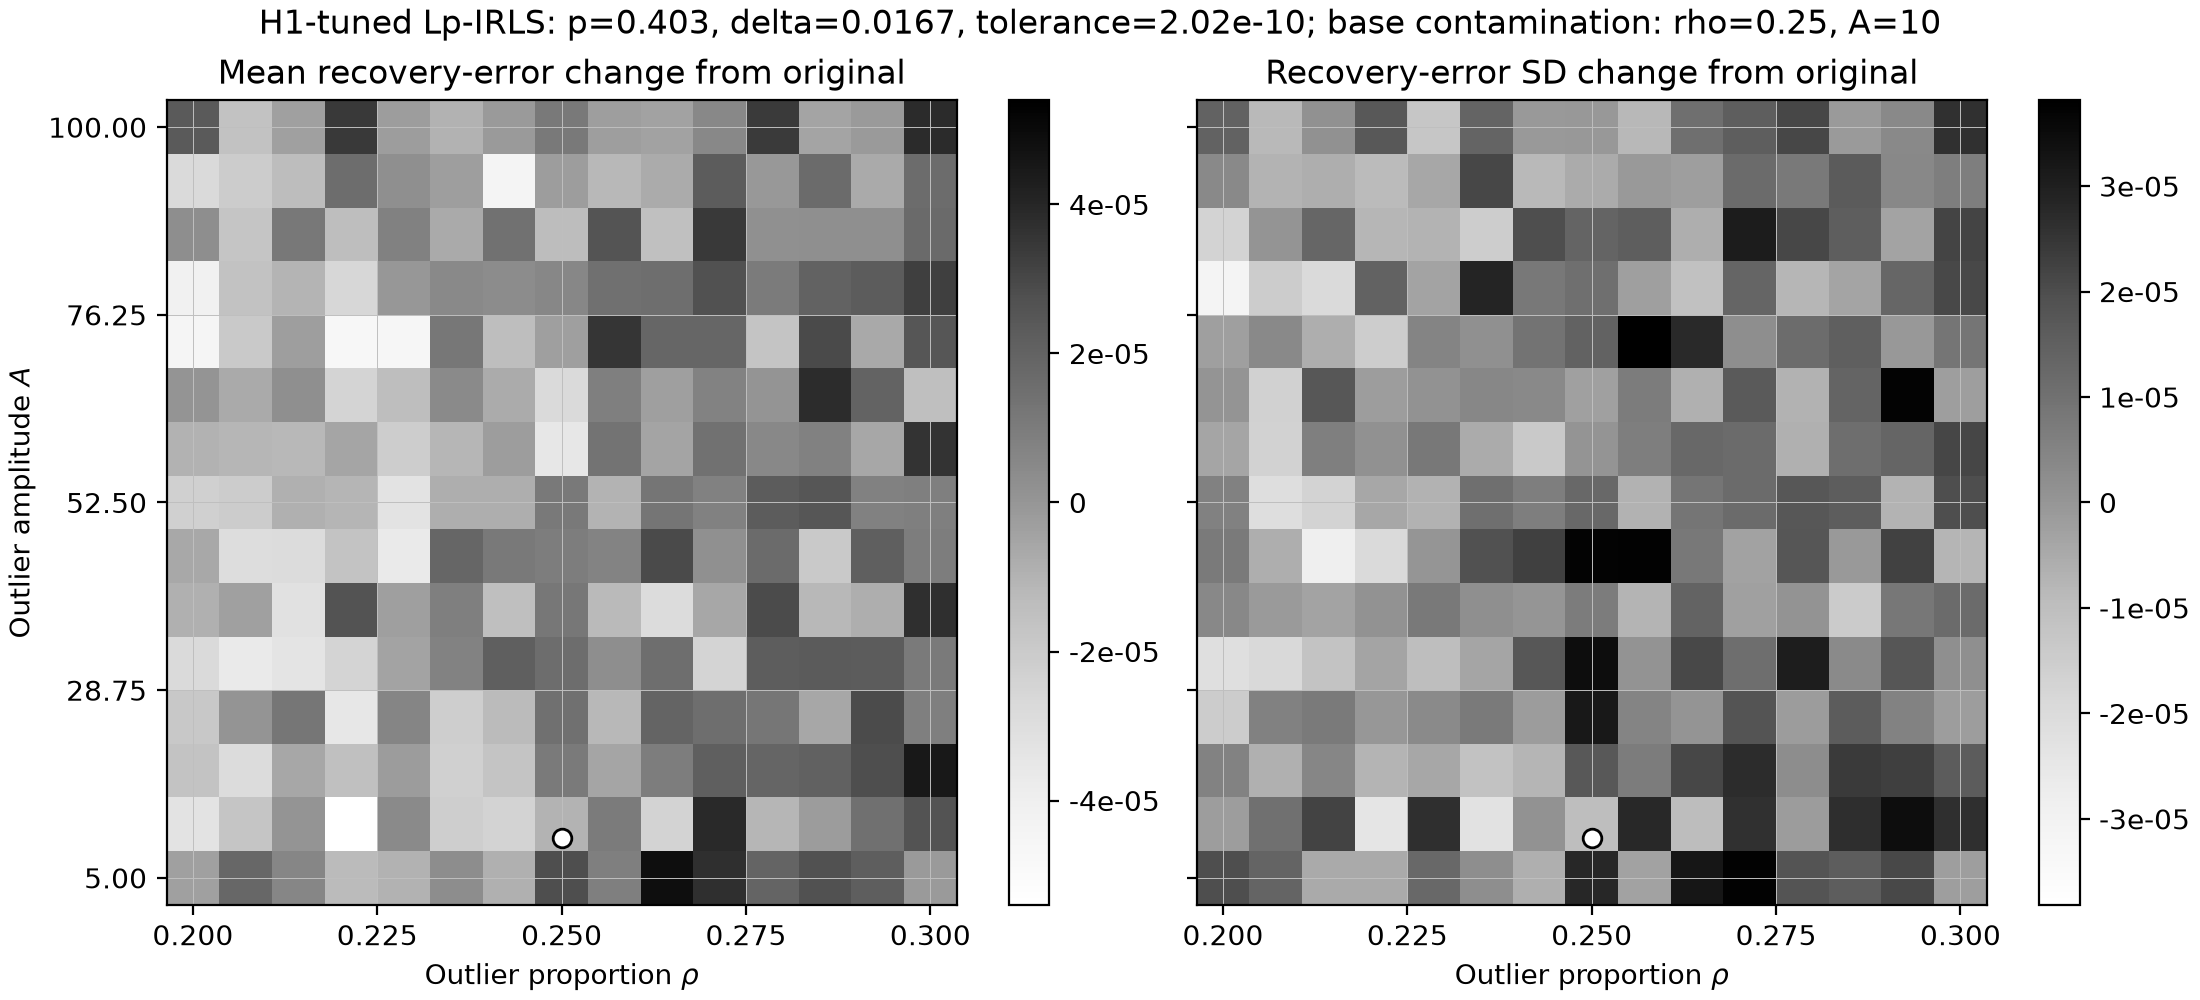
\includegraphics[width=\columnwidth]{../Assets/h4_comparison.png}
  \caption{Contamination-transfer experiment for the H1-tuned $L_p$-IRLS
  settings. Mean coefficient-recovery error and its standard deviation are
  compared across a $15\times15$ grid spanning $\rho=0.20$--$0.30$ and
  $A=5$--$100$. The heatmaps show changes relative to values bilinearly
  interpolated at the anchor setting $(\rho_0,A_0)=(0.25,10)$.}
  \label{fig:h4-contamination-transfer}
\end{figure}

\section{Hypothesis 5}
\label{sec:H5}

Hypothesis 5 tests whether a contamination regime can be estimated from the
observed sample and used to select $L_p$-IRLS settings without knowing the
generating coefficients. The data generator adds independent Gaussian clean
noise and, with probability $\rho$, a Gaussian contamination perturbation with
standard deviation $A$. After a preliminary robust fit, the residual
distribution is therefore approximated by the zero-mean scale mixture
\[
  f(r) \approx (1-\rho)\,\mathcal{N}(r;0,\sigma^2)
       + \rho\,\mathcal{N}(r;0,\sigma^2+A^2).
\]
The two component means are fixed at zero to reflect the symmetric
contamination model. We fit the component weights and variances by
expectation-maximization, then recover the contamination estimates as the
broad-component weight $\hat{\rho}$ and
$\hat{A}=\sqrt{\max(0,\hat{\sigma}_{\mathrm{broad}}^2-
\hat{\sigma}_{\mathrm{clean}}^2)}$.

The preliminary coefficients are fitted by Huber regression. Its threshold is
adaptively set to $1.345$ times a median-absolute-deviation estimate of the
residual scale, and the scale and fit are updated four times at most. The
Huber residuals are then used for the mixture fit. Rather than quantizing the
estimated pair $(\hat{\rho},\hat{A})$ to the nearest grid point, we use it as
a continuous input to bilinearly interpolate the oracle settings. The map is
interpolated linearly in $\rho$ and $\log A$; $p$ is interpolated directly,
while the positive parameters $\delta$ and $\tau$ are interpolated in log
space. Estimates outside the calibrated range are clipped to its boundary.
For comparison, we also evaluate a nearest-grid lookup. The $3\times3$ oracle
grid has $\rho\in\{0.20,0.25,0.30\}$ and $A\in\{5,10,20\}$.

At each grid point, a candidate-set oracle map is constructed by evaluating
15 settings sampled from the H1 Bayesian-optimization evaluations. The setting
with the lowest mean coefficient-recovery error over 20 independently seeded
tuning samples is retained for that regime. The evaluation uses a separate 100
samples per regime and compares five procedures: adaptive Huber; $L_p$-IRLS
selected by interpolating at the estimated regime; nearest-grid lookup using
the same estimates; the interpolated map queried with the true regime; and the
fixed H1 anchor setting. The true-regime interpolation is an oracle reference,
not a deployable method, because its construction uses the known generating
coefficients to score candidates. All methods are evaluated by
$\|\hat{\boldsymbol{\beta}}-\boldsymbol{\beta}\|_2$.

The mixture estimates were close to the generating values over the 900
evaluation samples: the mean absolute error in $\hat{\rho}$ was $0.0111$, the
mean relative absolute error in $\hat{A}$ was $3.86\%$, and the mean estimate
of $\sigma$ was $0.01001$ (the generating value is $0.01$). Nearest-grid lookup
selected the exact generating grid point in $94.8\%$ of samples.
Table~\ref{tab:h5-results} reports pooled recovery errors across all nine
regimes. Continuous use of the estimated pair reduced mean error by about 4.0\%
relative to nearest-grid lookup and was close to the true-regime interpolated
reference. This is consistent with avoiding quantization of the estimates.
However, the fixed H1 setting still had the lowest pooled mean error, so the
experiment does not show that regime estimation improves on reusing that
anchor for these particular regimes.

\begin{table}[H]
  \centering
  \caption{Hypothesis 5 coefficient-recovery error over 900 evaluation samples
  per method. Values are mean $\pm$ standard deviation.}
  \label{tab:h5-results}
  \scriptsize
  \resizebox{\columnwidth}{!}{%
  \begin{tabular}{lcc}
    \toprule
    Method & Mean error & Standard deviation \\
    \midrule
    Adaptive Huber & $6.718\times10^{-4}$ & $3.672\times10^{-4}$ \\
    Estimated, interpolated $L_p$ & $4.766\times10^{-4}$ & $2.426\times10^{-4}$ \\
    Estimated, nearest-grid $L_p$ & $4.965\times10^{-4}$ & $2.583\times10^{-4}$ \\
    True-regime interpolated $L_p$ & $4.981\times10^{-4}$ & $2.579\times10^{-4}$ \\
    H1 anchor $L_p$ & $4.464\times10^{-4}$ & $2.280\times10^{-4}$ \\
    \bottomrule
  \end{tabular}
  }
\end{table}

Using Huber to estimate the regime and then fitting another robust estimator
is not, by itself, a practical advantage: it requires two robust fits, and
Huber alone is already a reasonable alternative. The potential benefit is the
data-driven selection of $L_p$ settings when that estimator is desired and the
contamination regime is not known. The regime-specific map can be calibrated
offline and reused, avoiding a full parameter search for each new sample; a
robust preliminary fit supplies residuals without requiring the true
coefficients. The present experiment is a proof of concept for this workflow,
not evidence that it is preferable to Huber or to the H1 anchor. Its estimates
also rely on symmetric, two-scale Gaussian contamination, and should not be
assumed to transfer to other outlier distributions without further testing.

\begin{figure}[H]
  \centering
  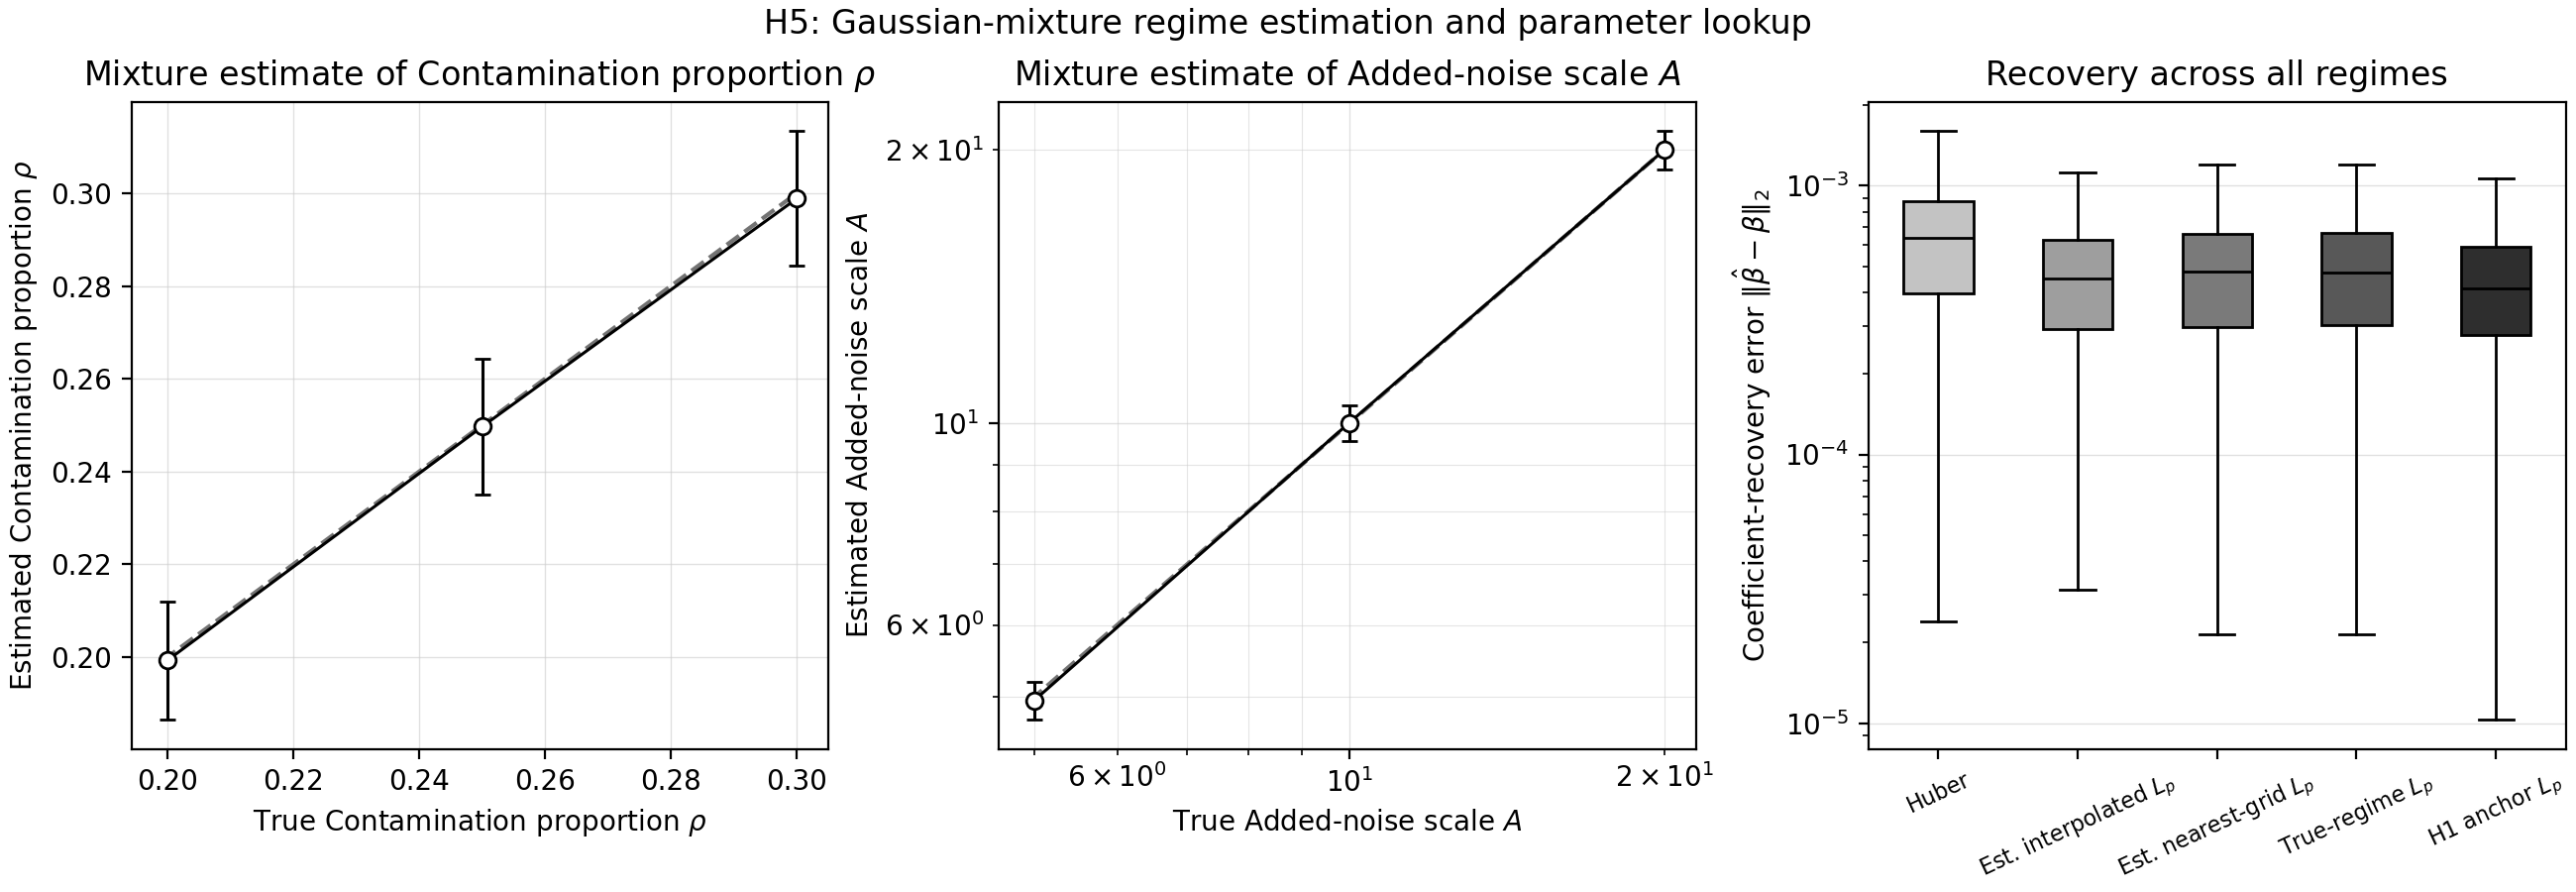
\includegraphics[width=\columnwidth]{../Assets/h5_comparison.png}
  \caption{Hypothesis 5 results. The first two panels compare estimated and
  true contamination proportion and added-noise scale; points show means and
  error bars show $\pm1$ standard deviation across replicates. The final panel
  compares coefficient-recovery errors for adaptive Huber, estimated-regime
  continuous interpolation, estimated-regime nearest-grid lookup, true-regime
  interpolation, and the fixed H1 anchor over all nine regimes.}
  \label{fig:h5-results}
\end{figure}

% ---------- References ----------
\small
\bibliographystyle{plain}
\bibliography{references}   % create references.bib
\normalsize

\end{multicols}
\end{document}